\chapter{Guia de notación}
\label{ape:notacion}

A continuación describiremos brevemente la notación utilizada en los diagramas utilizados a lo largo de este trabajo para modelar estructuras de clase y relaciones estáticas entre éstas.

\section{Diagrama de clases}

En la figura \ref{fig:png_arquitectura} podemos observar la notación utilizada para modelar tanto clases concretas como abstractas. Una clase se denota por un rectángulo con el nombre de la clase en la parte superior. En el caso de tratarse de una clase abstracta encontraremos el nombre en cursiva y la flecha que une a la misma con la clase concreta que la implementa estará graficada mediante una línea punteada. Por otro lado, la línea que une a una subclase con la clase padre de la cual hereda estará dibujada utilizando una línea continua. Abajo del nombre de la clase pueden aparecer las operaciones o métodos de la misma y también las variables de clase que pudiese tener; para diferenciar entre éstos, antecederemos el signo $+$ al nombre de las operaciones, mientras que utilizaremos un signo $-$ para indicar las variables de clase. La información del tipo de datos de retorno de una operación así como el de los argumentos del mismo y de las variables de instancia se encuentra especificado en cada uno de los casos. 

\begin{figure}[H]
  	\centering
	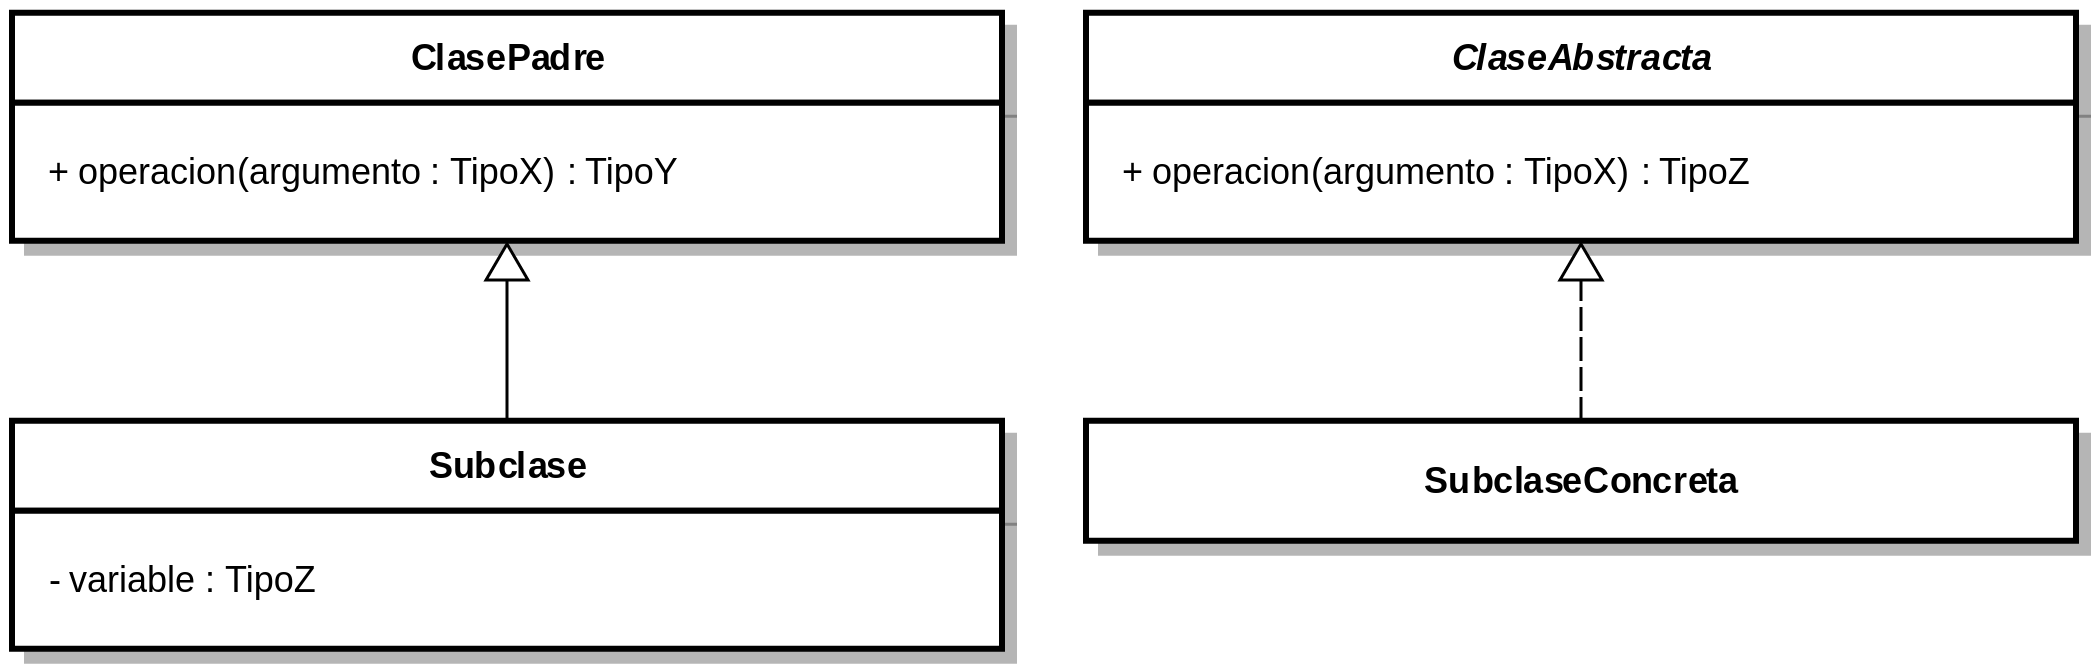
\includegraphics[scale=0.17]{img/ref_clases.png}
	\caption{Diagramas de clase}
  	\label{fig:png_arquitectura}
\end{figure}

En la figura \ref{fig:png_arquitectura} podemos ver la notación usada para indicar distintas referencias entre clases. Utilizamos una línea con un rombo blanco en el otro extremo para indicar agregación (en este caso \textbf{ClaseConcreta} tiene una referencia a \textbf{ClaseA} y este último puede existir de forma independiente de A). Por otro lado, utilizamos un rombo negro para indicar composición (en este caso caso \textbf{ClaseConcreta} tiene una referencia a \textbf{ClaseC} y este último no puede existir por separado). En ambos casos, es posible indicar la cardinalidad de estas relaciones como se muestra en la figura. Finalmente, en algunos diagramas del trabajo se puede ver una flecha con línea de puntos y el texto \emph{uses}, esto indica que una clase hace uso de una o mas operaciónes de la otra, se diferencia de la composición y agregación ya que no hace referenca a ningún objeto. Lo utilizamos, por ejemplo, para diferenciar las llamadas a un método estático de una libreria.

\begin{figure}[H]
  	\centering
	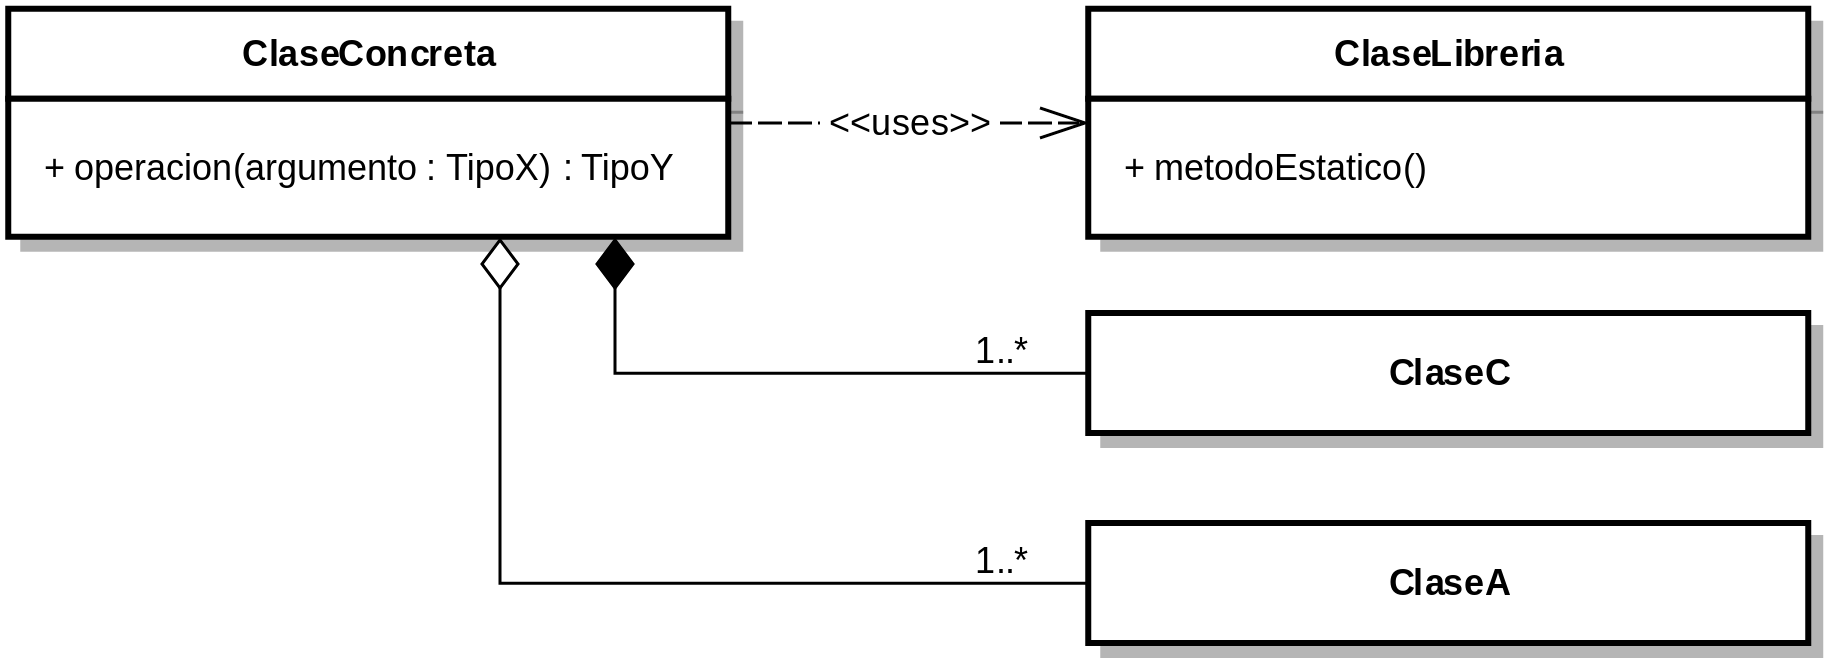
\includegraphics[scale=0.17]{img/ref_comp-agregation.png}
	\caption{Diagramas relacionese entre clases}
  	\label{fig:png_arquitectura}
\end{figure}


